\chapter{Considerações finais}

A presente dissertação tem como objetivo avaliar o desempenho de longo prazo de membranas comerciais no tratamento de água de produção via destilação por membranas. As análises serão realizadas em oito membranas com diferentes características morfológicas, incluindo material, suporte, diâmetro de poro e ângulo de contato.Os experimentos serão conduzidos em uma bancada equipada com um módulo AGMD, utilizando água de produção como corrente de alimentação, conforme as condições operacionais descritas no Capítulo 3. 

Os resultados obtidos serão comparados com o propósito de investigar a influência das diferentes características morfológicas das membranas sobre o desempenho do processo de tratamento da água de produção, considerando parâmetros como fluxo de permeado, estabilidade operacional e resistência ao molhamento.

Os resultados preliminares apresentados no Capítulo 4 evidenciam as principais características morfológicas das membranas avaliadas, incluindo diâmetro médio de poro , distribuição de poro, ângulo de contato e LEP. De modo geral, os resultados indicam que as membranas possuem potencial para aplicação em processos de destilação por membranas, em função de suas características hidrofóbicas. 

Em relação ao LEP, as membranas M4 e M6 apresentam maior probabilidade de molhamento, associada aos elevados diâmetros de poro observados. Além disso, verificou-se que as distribuições de poro das membranas diferem significativamente de uma distribuição normal. Dessa forma, será realizada uma análise estatística mais aprofundada, com o objetivo de determinar as incertezas associadas aos parâmetros avaliados de maneira mais representativa e confiável.

Por fim, ressalta-se que os materiais e equipamentos necessários para a conclusão da pesquisa encontram-se disponíveis no LabMEMS e em laboratórios parceiros. O cronograma para a realização da pesquisa é apresentado na figura \ref{fig:cronograma}.

\begin{figure}[H]
    \centering
    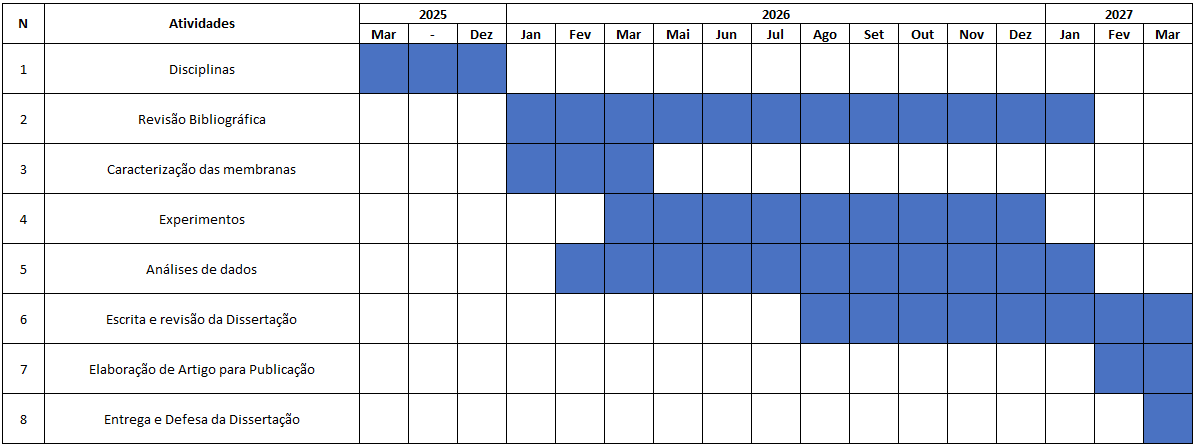
\includegraphics[angle=90, width=\textwidth, height=20cm, keepaspectratio]{cronograma.png}
    \caption{Cronograma da dissertação.}
    \label{fig:cronograma}
\end{figure}